\subsection{Estimated Speedup Factor}
BRRRRRR GO FAST!
%\begin{figure}[H]
    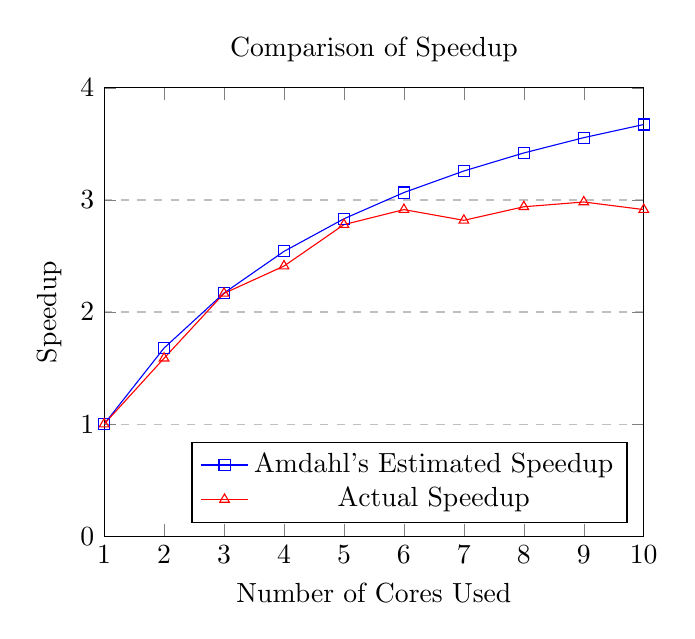
\begin{tikzpicture}
    \begin{axis}[
        title={Comparison of Speedup},
        xlabel={Number of Cores Used},
        ylabel={Speedup},
        xmin=1, xmax=10,
        ymin=0, ymax=4,
        xtick={1,2,3,4,5,6,7,8,9,10},
        ytick={0,1,2,3,4},
        legend pos=south east,
        ymajorgrids=true,
        grid style=dashed,
    ]
    
    \addplot[
        color=blue,
        mark=square,
        ]
        coordinates {
        (1,1)(2,1.6787346222)(3,2.1695941855)(4,2.5411013569)(5,2.8320683114)(6,3.0661245456)(7,3.2584795325)(8,3.4193663866)(9,3.5559232301)(10,3.6732810342)
        };
        \addlegendentry{Amdahl's Estimated Speedup}
    
    \addplot[
        color=red,
        mark=triangle,
        ]
        coordinates {
        (1,1)(2,1.5877659574)(3,2.1663138796)(4,2.4100925147)(5,2.7799767171)(6,2.9139719341)(7,2.8182533438)(8,2.9390769231)(9,2.9818938606)(10,2.9139719341)
        };
        \addlegendentry{Actual Speedup}
    
    \end{axis}
    \end{tikzpicture}
    \caption{A comparison on the estimated speedup from Amdahl's law and the actual Speedup for 3DM on DUT 2}\label{fig:amdahls}
%\end{figure}



% To compare the predicted speedup from Amdahl's Law to the actual speedup achieved, you'll need to follow these steps:

%     Run the benchmark on a single core: Execute the original, non-parallelized version of your program on a single core or processor, and measure its execution time (T_serial).

%     Determine the fractions S and P: Analyze your code to identify the serial (S) and parallel (P) portions, as previously discussed.

%     Predict the speedup using Amdahl's Law: Use the formula Sp = 1 / (S + (P / N)) to predict the potential speedup (Sp_predicted) when using N cores (e.g., 10 cores in your example).

%     Implement the parallel version: Modify your code to incorporate parallelism using a suitable parallel programming model, as previously discussed.

%     Run the benchmark on multiple cores: Execute the parallelized version of your program on multiple cores (e.g., 10 cores), and measure its execution time (T_parallel).

%     Calculate the actual speedup: Divide the single-core execution time (T_serial) by the multi-core execution time (T_parallel) to obtain the actual speedup (Sp_actual), as previously discussed.

%     Compare the predicted and actual speedups: Analyze the difference between the predicted speedup (Sp_predicted) from Amdahl's Law and the actual speedup (Sp_actual) achieved by your parallelized program. This comparison can help you understand the efficiency of your parallelization efforts and identify any potential bottlenecks or areas for further optimization.




% From a 3DM, DUT 2 using 10 cores.
% start: 0.06699943542480469
% end: 41.49199676513672
% Time total = Ttotal = 41,4249973297

% Time serial = Ts
% ~ Ts start: 0.06699943542480469
% ~ Ts end: 13.687000274658203

% ~ Ts start: 32.38800048828125
% ~ Ts end: 41.49199676513672
% ~Ts: (13,687000274658203 - 0,06699943542480469) + (41,49199676513672 - 32,38800048828125) = 22,7239971161


% Fraction of the serial portion (S)
% S = Ts / Ttotal = 22,7239971161 / 41,4249973297 = 0,5485576000

% Fraction of the parallel portion (P).
% P = 1 - S = 1 - 0,5485576000 = 0,4514424


% Compute the speedup factor (Sp) for the task using Amdahl's Law formula:

% Sp = 1 / (S + (P / N))
% Sp = 1 / (0,5485576000 + (0,4514424 / 10)) = 1,6843471464
% where Sp is the speedup factor, N is the number of processing elements or cores, and S and P are the fractions of the task that are serial and parallel, respectively.


% %%%%%%%%
% Parallel start on 1 core : 19 sec
% Parallel end on 1 core: 130.8 sec
% Benchmark end on 1 core: 141.3 sec

% Ts = 19 + (141,3 - 130,8) = 29,5

% Fraction of the serial portion (S)
% S = 29,5 / 141,3 = 0,2087756546

% Fraction of the parallel portion (P).
% P = 1 - 0,2087756546 = 0,7912243454

% %%%%
% Estimated speed up factor (Sp) for 2 cores
% Sp = 1 / (S + (P / N)) = 
% 1 / (0,2087756546 + (0,7912243454 / 2)) = 1,6545667448

% Actual speed up factor for 2 cores

% Benchmark end on 2 cores: 84,6 sec
% Sp = T_single / T_multi = 141,3 / 84,6 = 1,6702127660

% %%%%

% Estimated speed up factor (Sp) for 3 cores
% Sp = 1 / (0,2087756546 + (0,7912243454 / 3)) = 2,1163255118

% Actual speed up factor for 3 cores

% Benchmark end on 3 cores: 64,2 sec
% Sp = T_single / T_multi = 141,3 / 64,2 = 2,2009345794

% %%%%

% Estimated speed up factor (Sp) for 4 cores
% Sp = 1 / (0,2087756546 + (0,7912243454 / 4)) = 2,4595300263

% Actual speed up factor for 4 cores

% Benchmark end on 4 cores: 55,8 sec
% Sp = T_single / T_multi = 141,3 / 55,8 = 2,5322580645

% %%%%

% Estimated speed up factor (Sp) for 5 cores
% Sp = 1 / (0,2087756546 + (0,7912243454 / 5)) = 2,7246432706

% Actual speed up factor for 5 cores

% Benchmark end on 5 cores: 50,4 sec
% Sp = T_single / T_multi = 141,3 / 50,4 = 2,8035714286

% %%%%

% Estimated speed up factor (Sp) for 6 cores
% Sp = 1 / (0,2087756546 + (0,7912243454 / 6)) = 2,9355955681

% Actual speed up factor for 6 cores

% Benchmark end on 6 cores: 48,2 sec
% Sp = T_single / T_multi = 141,3 / 48,2 = 2,9315352697

% %%%%

% Estimated speed up factor (Sp) for 7 cores
% Sp = 1 / (0,2087756546 + (0,7912243454 / 7)) = 3,1074458061

% Actual speed up factor for 7 cores

% Benchmark end on 7 cores: 46,6 sec
% Sp = T_single / T_multi = 141,3 / 46,6 = 3,0321888412

% %%%%

% Estimated speed up factor (Sp) for 8 cores
% Sp = 1 / (0,2087756546 + (0,7912243454 / 8)) = 3,2501437611

% Actual speed up factor for 8 cores

% Benchmark end on 8 cores: 47,2 sec
% Sp = T_single / T_multi = 141,3 / 47,2 = 2,9936440678

% %%%%

% Estimated speed up factor (Sp) for 9 cores
% Sp = 1 / (0,2087756546 + (0,7912243454 / 9)) = 3,3705274321

% Actual speed up factor for 9 cores

% Benchmark end on 9 cores: 47,5 sec
% Sp = T_single / T_multi = 141,3 / 47,5 = 2,9747368421

% %%%
% Estimated speed up factor (Sp) for 10 cores
% Sp =  1 / (0,2087756546 + (0,7912243454 / 10)) = 3,4734513278

% Actual speed up factor for 2 cores

% Benchmark end on 10 cores: 47,8 sec
% Sp = T_single / T_multi = 141,3 / 47,8 = 2,9560669456